\begin{figure}[t!]
    \begin{subfigure}[b]{0.5\textwidth}
    \centering
    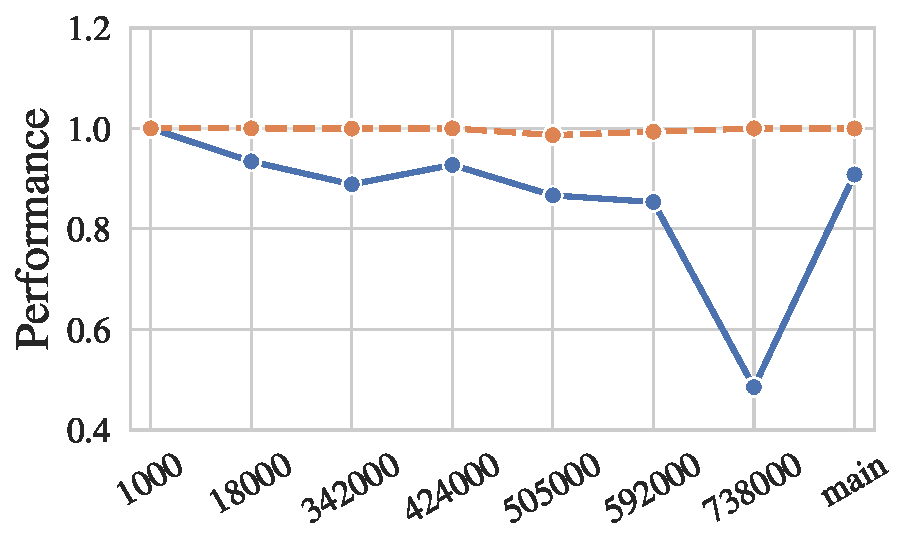
\includegraphics[width=0.7\columnwidth]{figures/fig_files/ood/sft_evalqqp-trainpaws_main_display.pdf}
        \caption{Paws $\rightarrow$ QQP}
        \label{fig:ood:detrimental}
    \end{subfigure}%
    \\
    \begin{subfigure}[b]{0.5\textwidth}
        \centering
    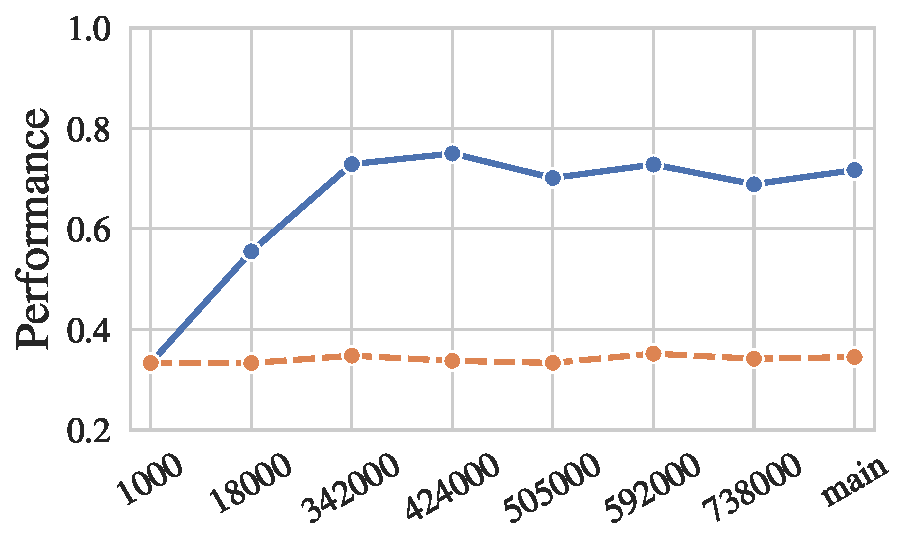
\includegraphics[width=0.7\columnwidth]{figures/fig_files/ood/sft_evalgpt3nli-trainmnli_main_display.pdf}
        \caption{MNLI $\rightarrow$ GPT3NLI}
        \label{fig:ood:beneficial}
    \end{subfigure}
    \caption{Example of out-of-domain performance for fine-tuned models. The \textcolor{snsblue}{\textbf{solid blue}} line represents the fine-tuned checkpoint evaluated on an out-of-domain dataset, and the \textcolor{snsorange}{\textbf{dashed orange}} line represents the base checkpoint where the model is not fine-tuned. Figure~\ref{fig:ood:detrimental} shows an example of fine-tuning hurting OOD performance, while Figure~\ref{fig:ood:beneficial} shows an example of fine-tuning boosting OOD performance as pre-traininng proceeds. }
    \label{fig:findings:ood}
\end{figure}